\documentclass[letterpaper, 10 pt, conference]{article} 
\usepackage[spanish]{babel}
\usepackage{amsmath,amssymb,amscd,amsthm} % variety of useful math macros
\usepackage[inner=1.5 cm, outer = 1.5 cm, top=1 cm, bottom = 1.5 cm]{geometry}
\usepackage{subcaption}
%For inserting graphics
\usepackage{graphicx}
\usepackage[dvipsnames]{xcolor}
\usepackage{listings}
\usepackage[utf8]{inputenc}
\usepackage{hyperref}
\usepackage{array, multirow}
\usepackage{pdfpages}
\begin{document}

%\newpage
\thispagestyle{empty}
\vspace{10 cm}
\begin{scshape}
\begin{center}
	{$\,$} \\[20 mm]
	{\Large{Universidad Autónoma de Nuevo León}} \\[5mm]
	{\large{Facultad de Ingeniería Mecánica y Eléctrica}} \\[5mm]
	{\large{Posgrado en Ciencias de la Ingeniería con Orientación en Nanotecnología}} \\[5 mm]
	\vskip16mm
	\begin{figure}[h!]
		\centering
		\begin{subfigure}{0.3\linewidth}
			\includegraphics[width=\linewidth]{imagen_2022-06-01_124754160.png}
		\end{subfigure}
		\hspace{15 mm}
		\begin{subfigure}{0.32\linewidth}
			\includegraphics[width=\linewidth]{fimelogo.jpg}
		\end{subfigure}
	\end{figure}
	\vskip16mm
	\begin{tabular}{p{11cm}}
		\centering
		{\large Portafolio de Evidencias}
	\end{tabular}
	\vskip7mm
	{de}\\[7mm]
	{\large Jorge Alejandro Torres Quintanilla}\\[3mm]
	{1642654}\\[7 mm]
	{para el curso de Simulación Computacional de Nanomateriales,}\\[3mm]
	{Dr. Virgilio González González en colaboración con Dra. Elisa Schaeffer Elisa Schaeffer.}\\[3mm]
	Segundo Semestre. Enero - Junio 2022. \\ [5 mm]
	\begin{table}[ht]
\centering

\begin{tabular}{|c|c|c|c|c|c|c|c|c|c|c|c|c|c|c|} 
 \hline
 \multicolumn{12}{|c|}{Práctica} & \multirow{2}{*}{T} & \multirow{2}{*}{P} & \multirow{2}{*}{C} \\
 \cline{1-12}
 $t_1$ & $t_2$ & $t_3$ & $t_4$ & $t_5$ & $t_6$ & $t_7$ & $t_8$ & $t_9$ & $t_{10}$ & $t_{11}$ & $t_{12}$ & & & \\
 \hline
 $7$ & $6$ & $6$ & $6$ & $7$ & $5$ & $6$ & $6$ & $8$ & $6$ & $8$ & $8$ & \multicolumn{1}{|c|}{79} & $3+3+3+1+0+5=15$ & \multicolumn{1}{|c|}{94}\\
 \hline
\end{tabular}
\label{Cuadro3}
\end{table}

\url{https://github.com/FeroxDeitas/Simulacion-Nano/tree/main/Tareas}
	\vfill
\end{center}
\end{scshape}

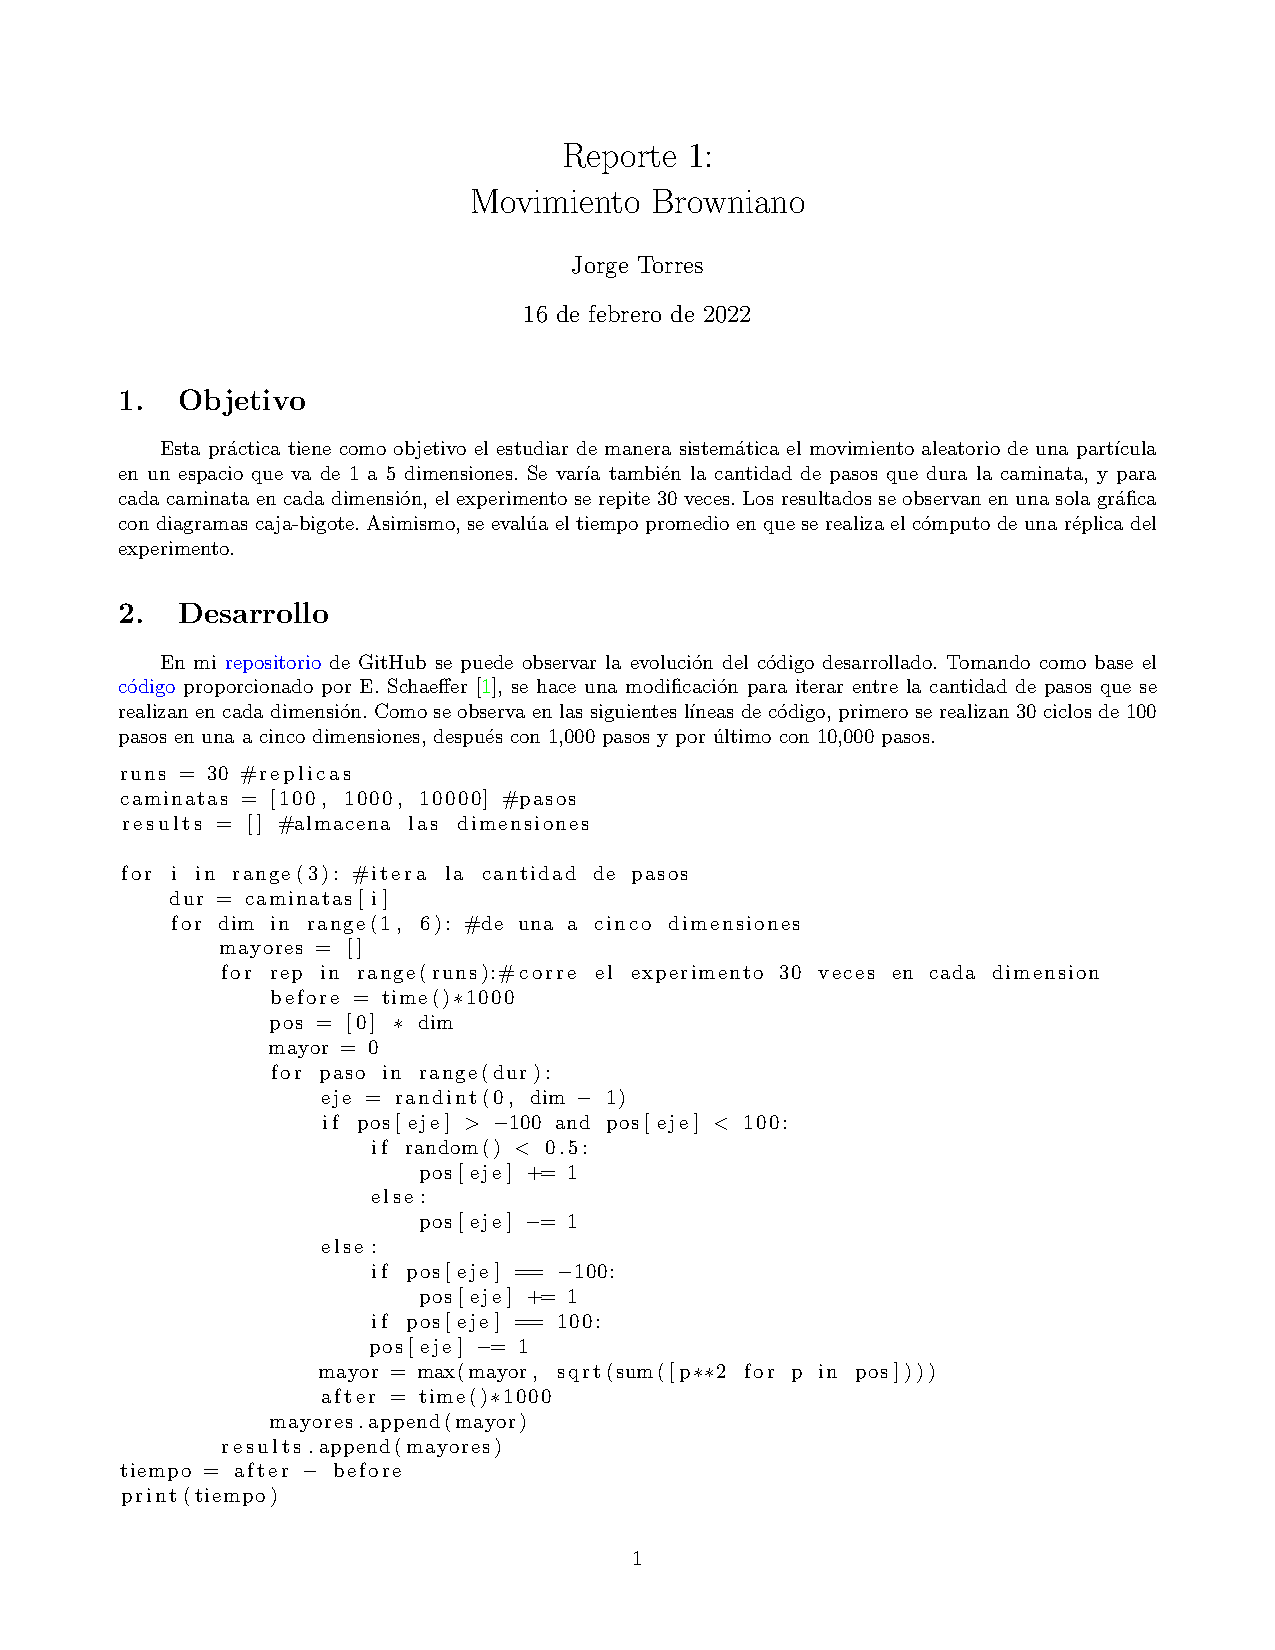
\includepdf[pages=-]{PDF_Tareas/Reporte_1.pdf}
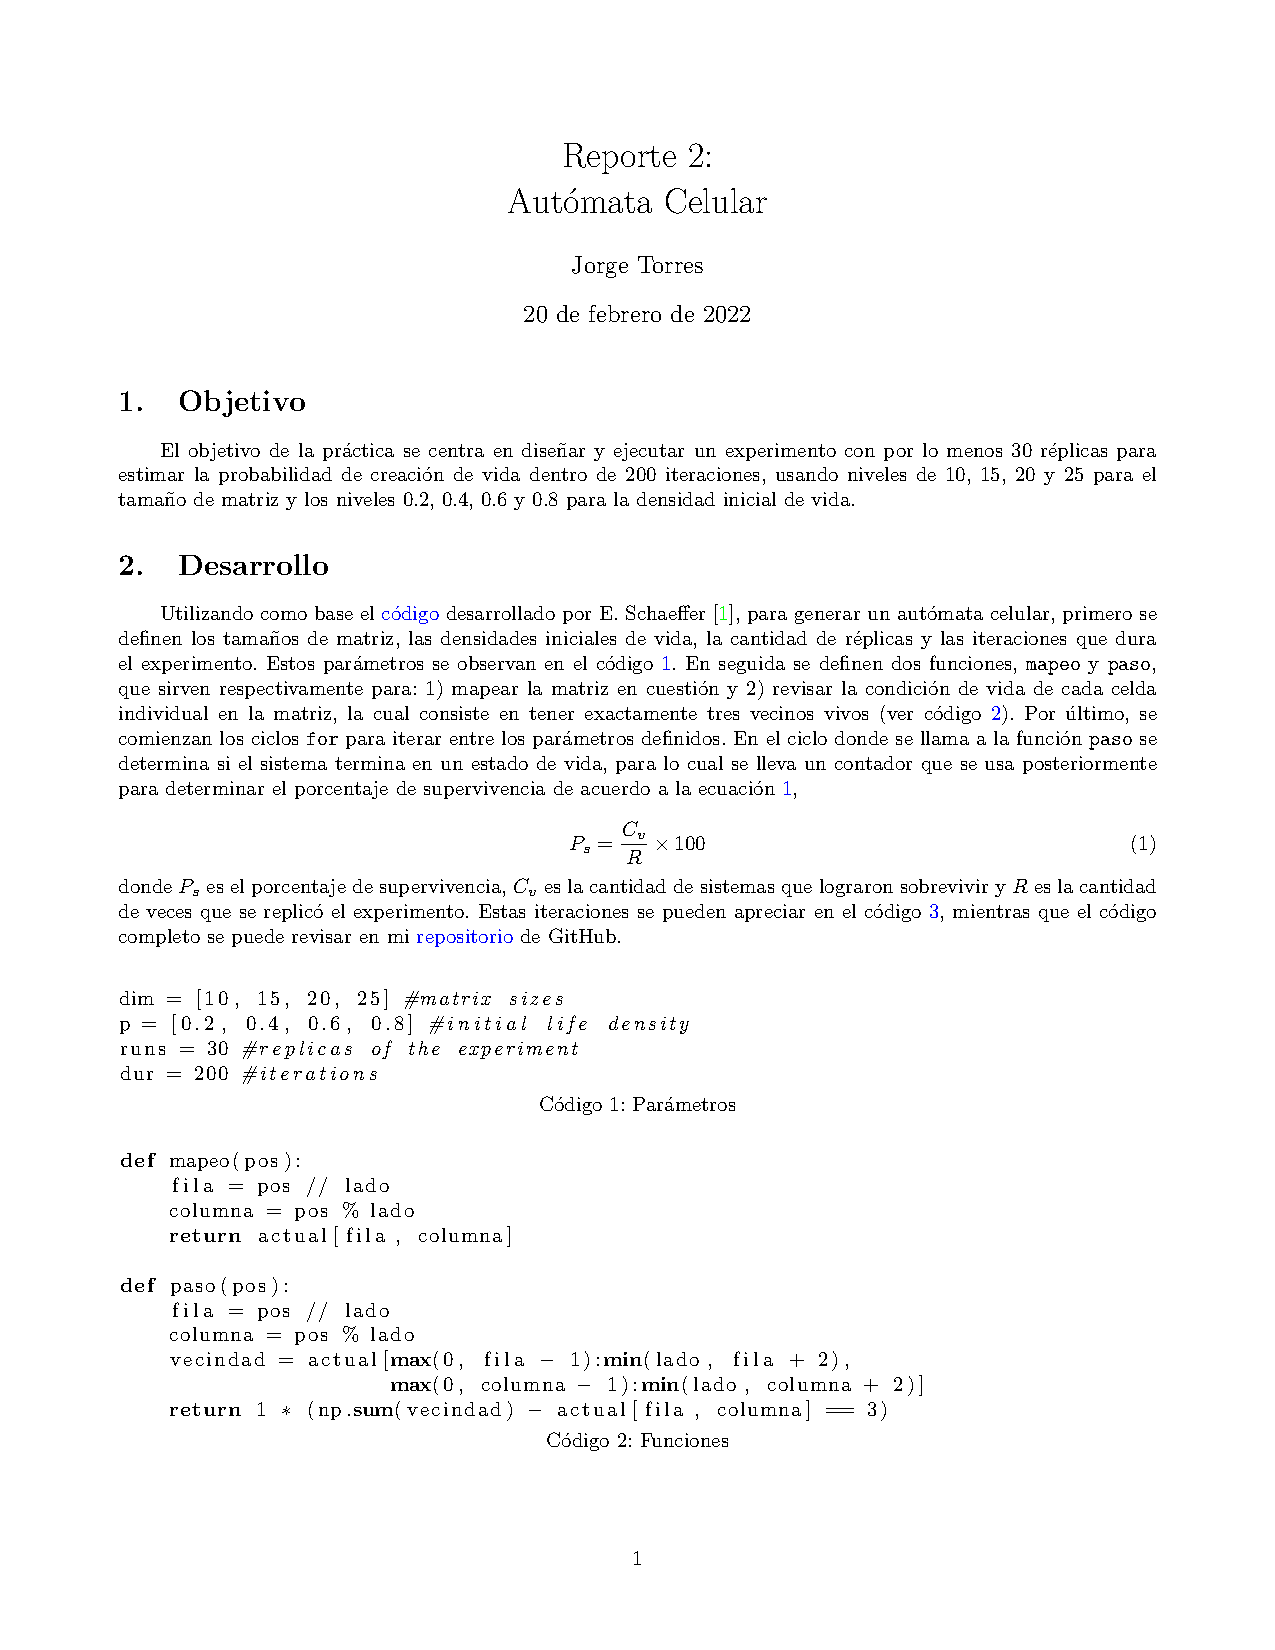
\includepdf[pages=-]{PDF_Tareas/Reporte_2.pdf}
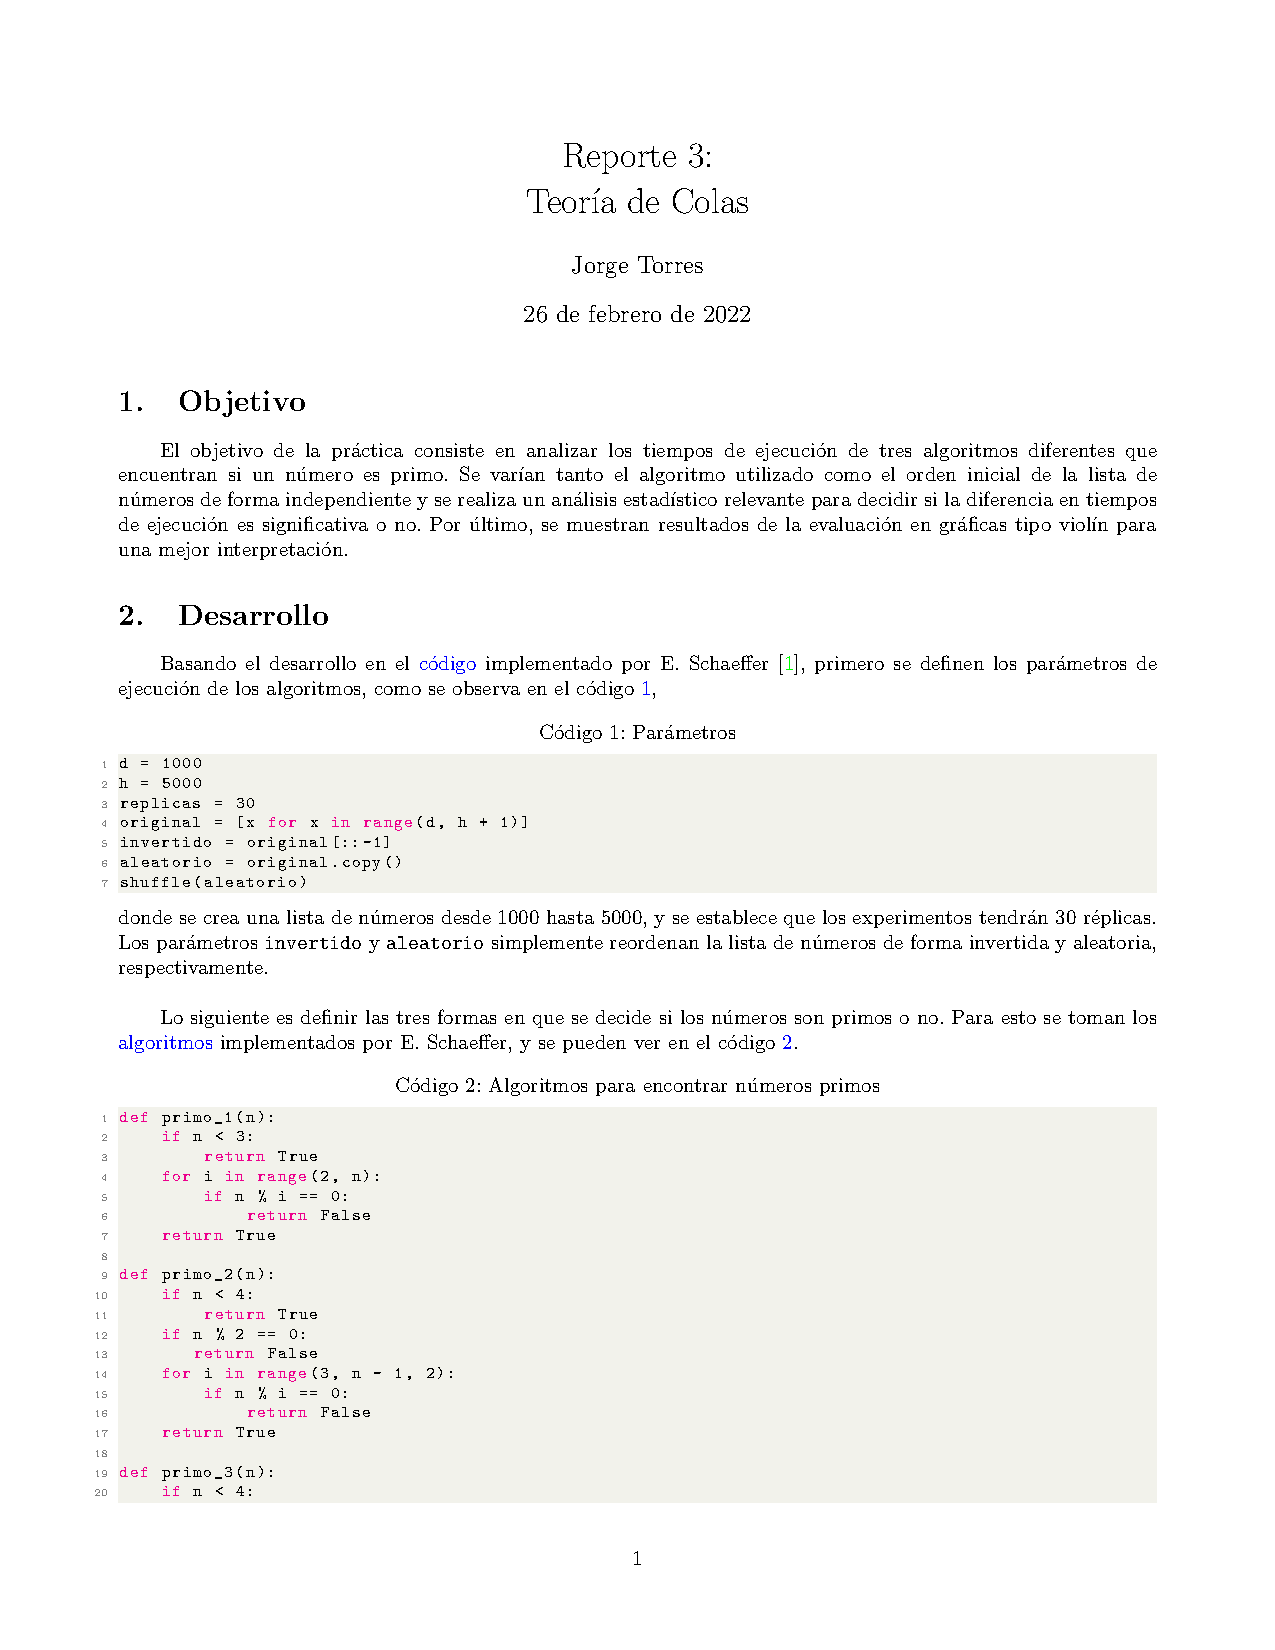
\includepdf[pages=-]{PDF_Tareas/Reporte_3.pdf}
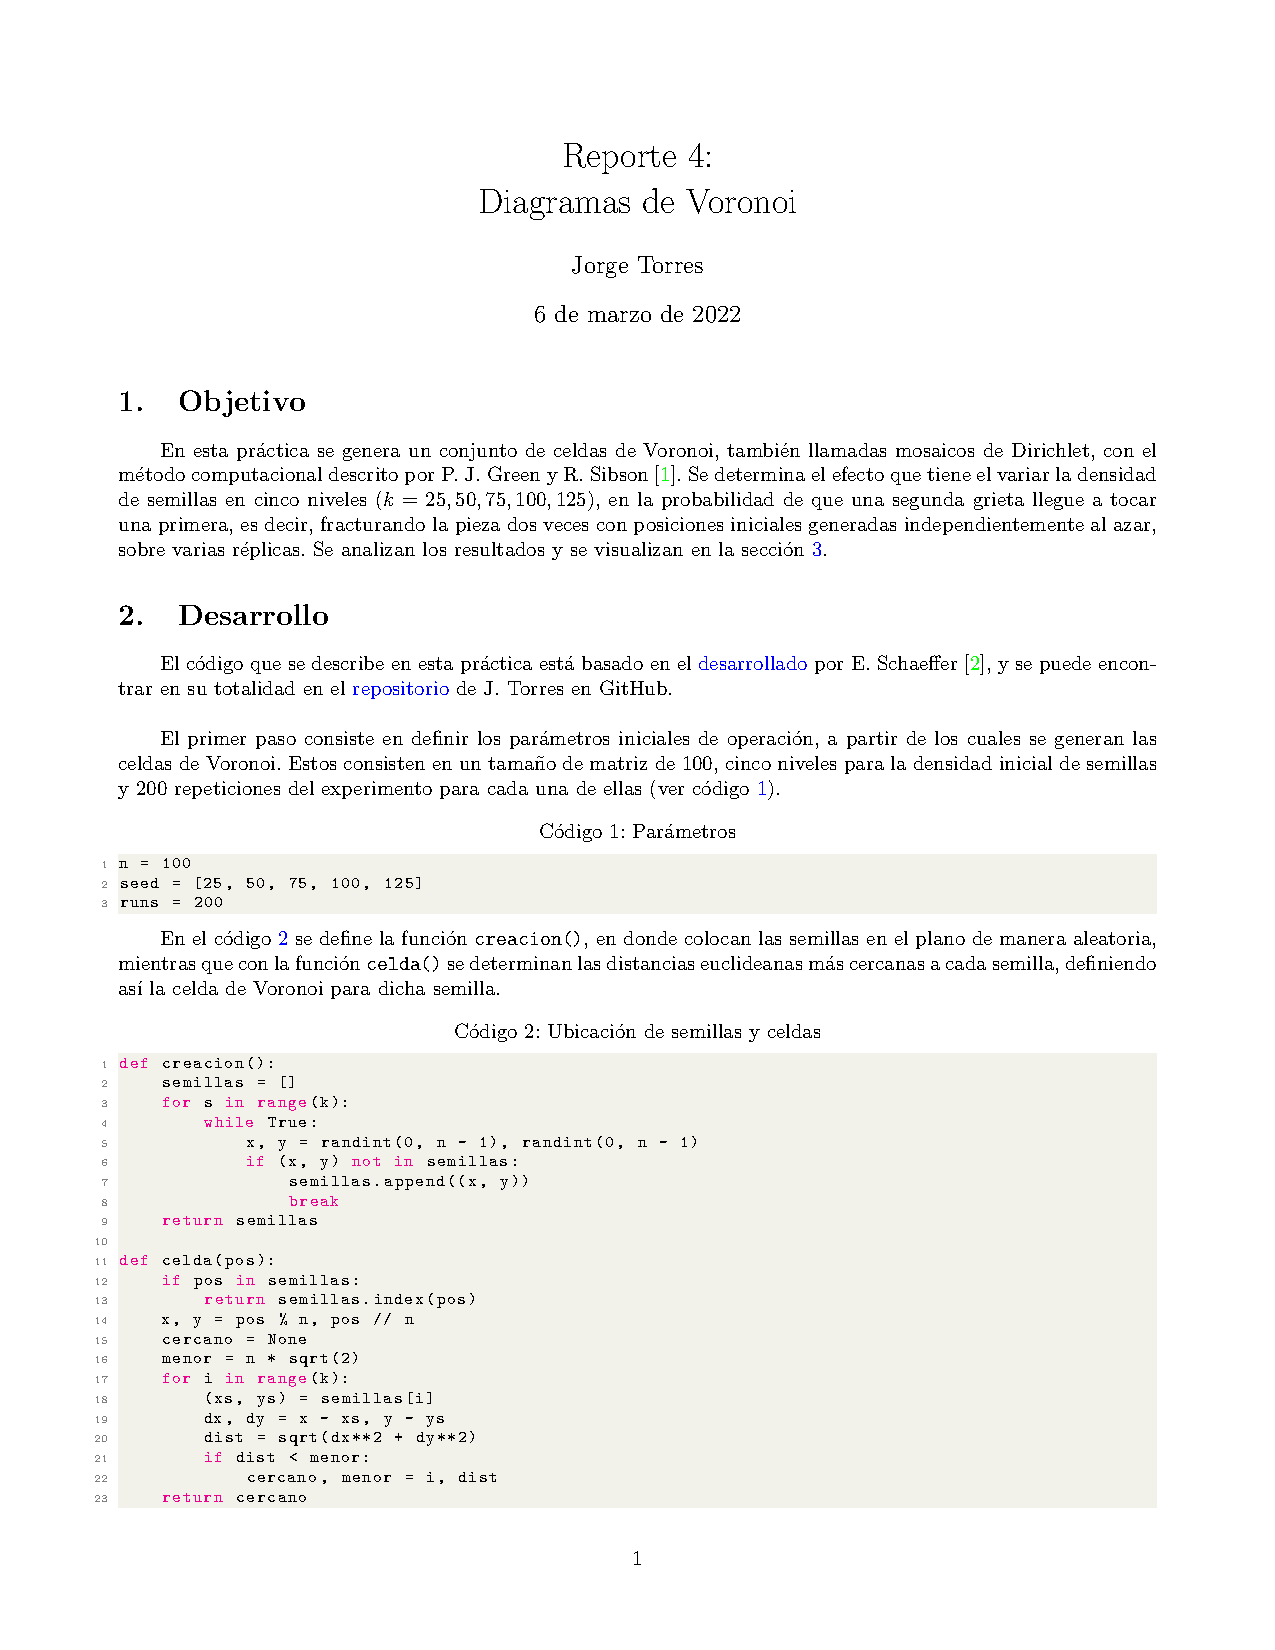
\includepdf[pages=-]{PDF_Tareas/Reporte_4.pdf}
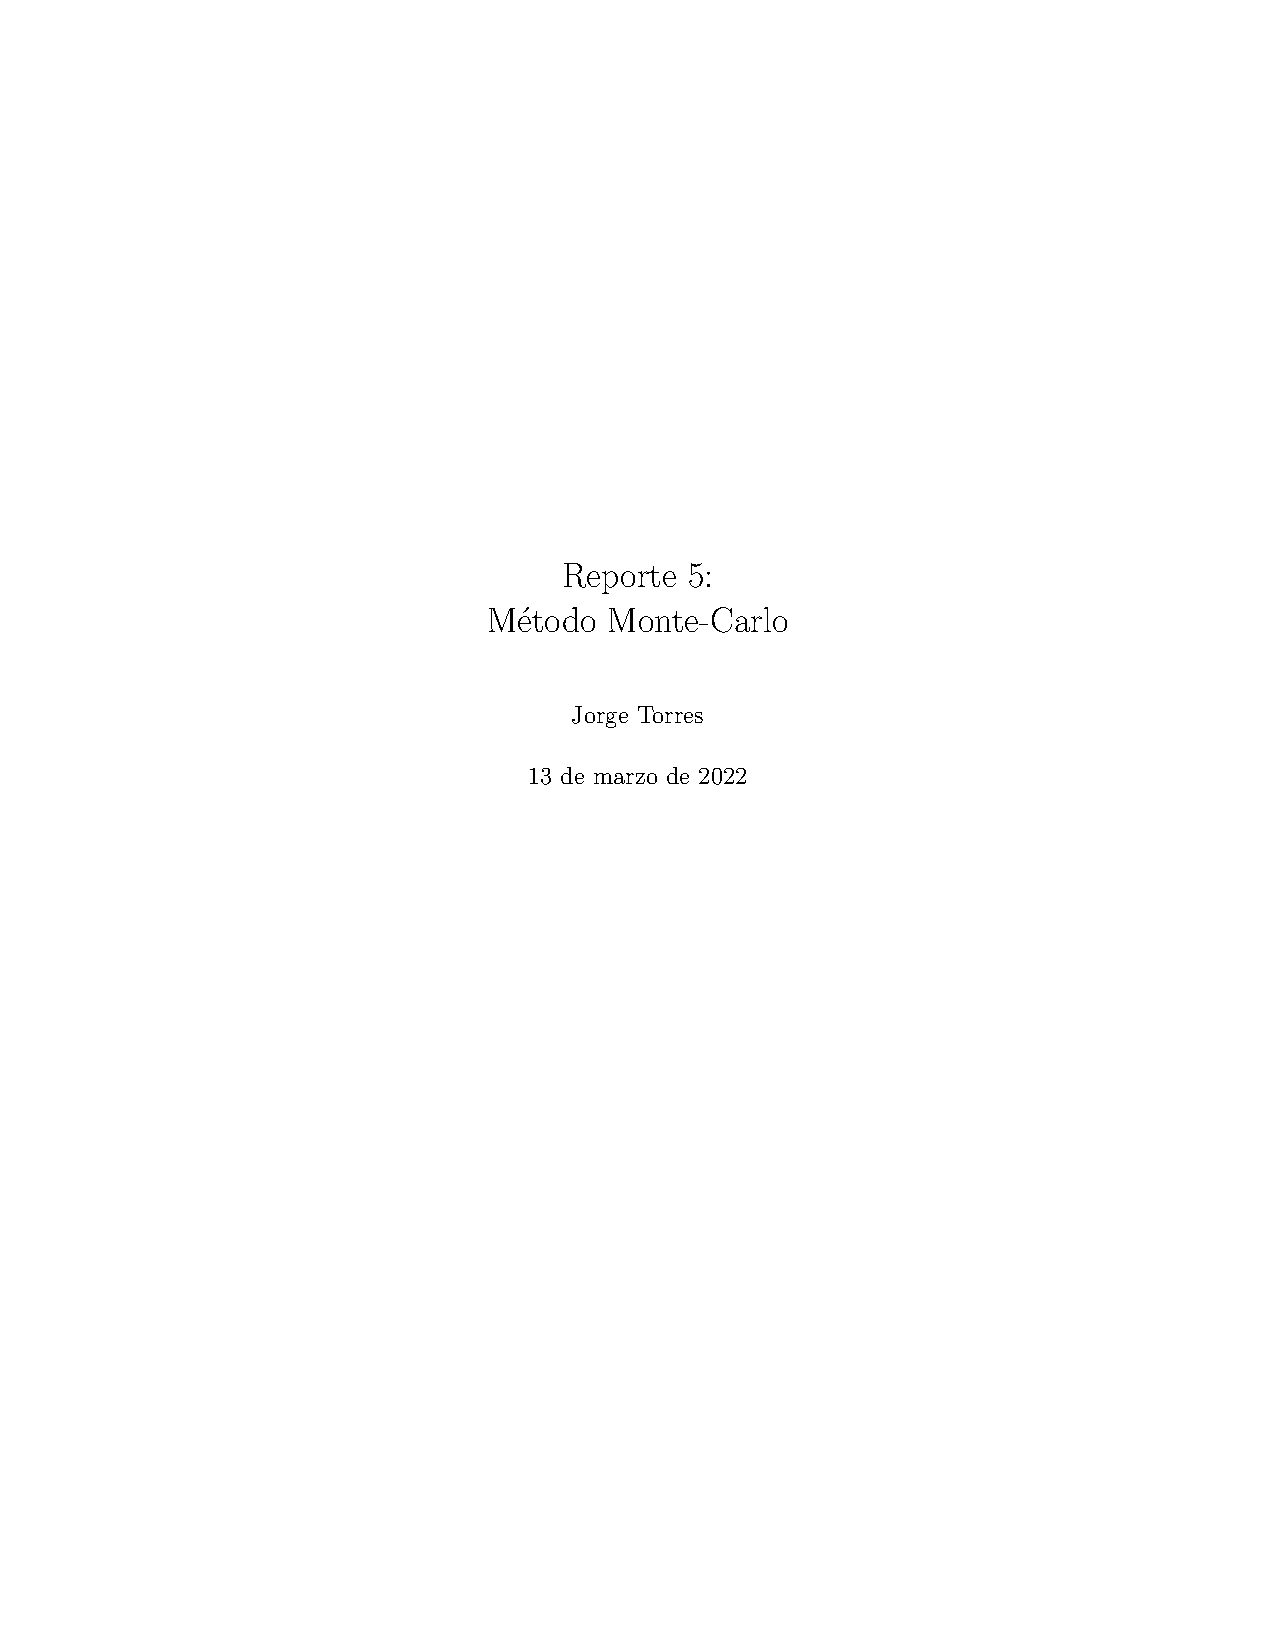
\includepdf[pages=-]{PDF_Tareas/Reporte_5.pdf}
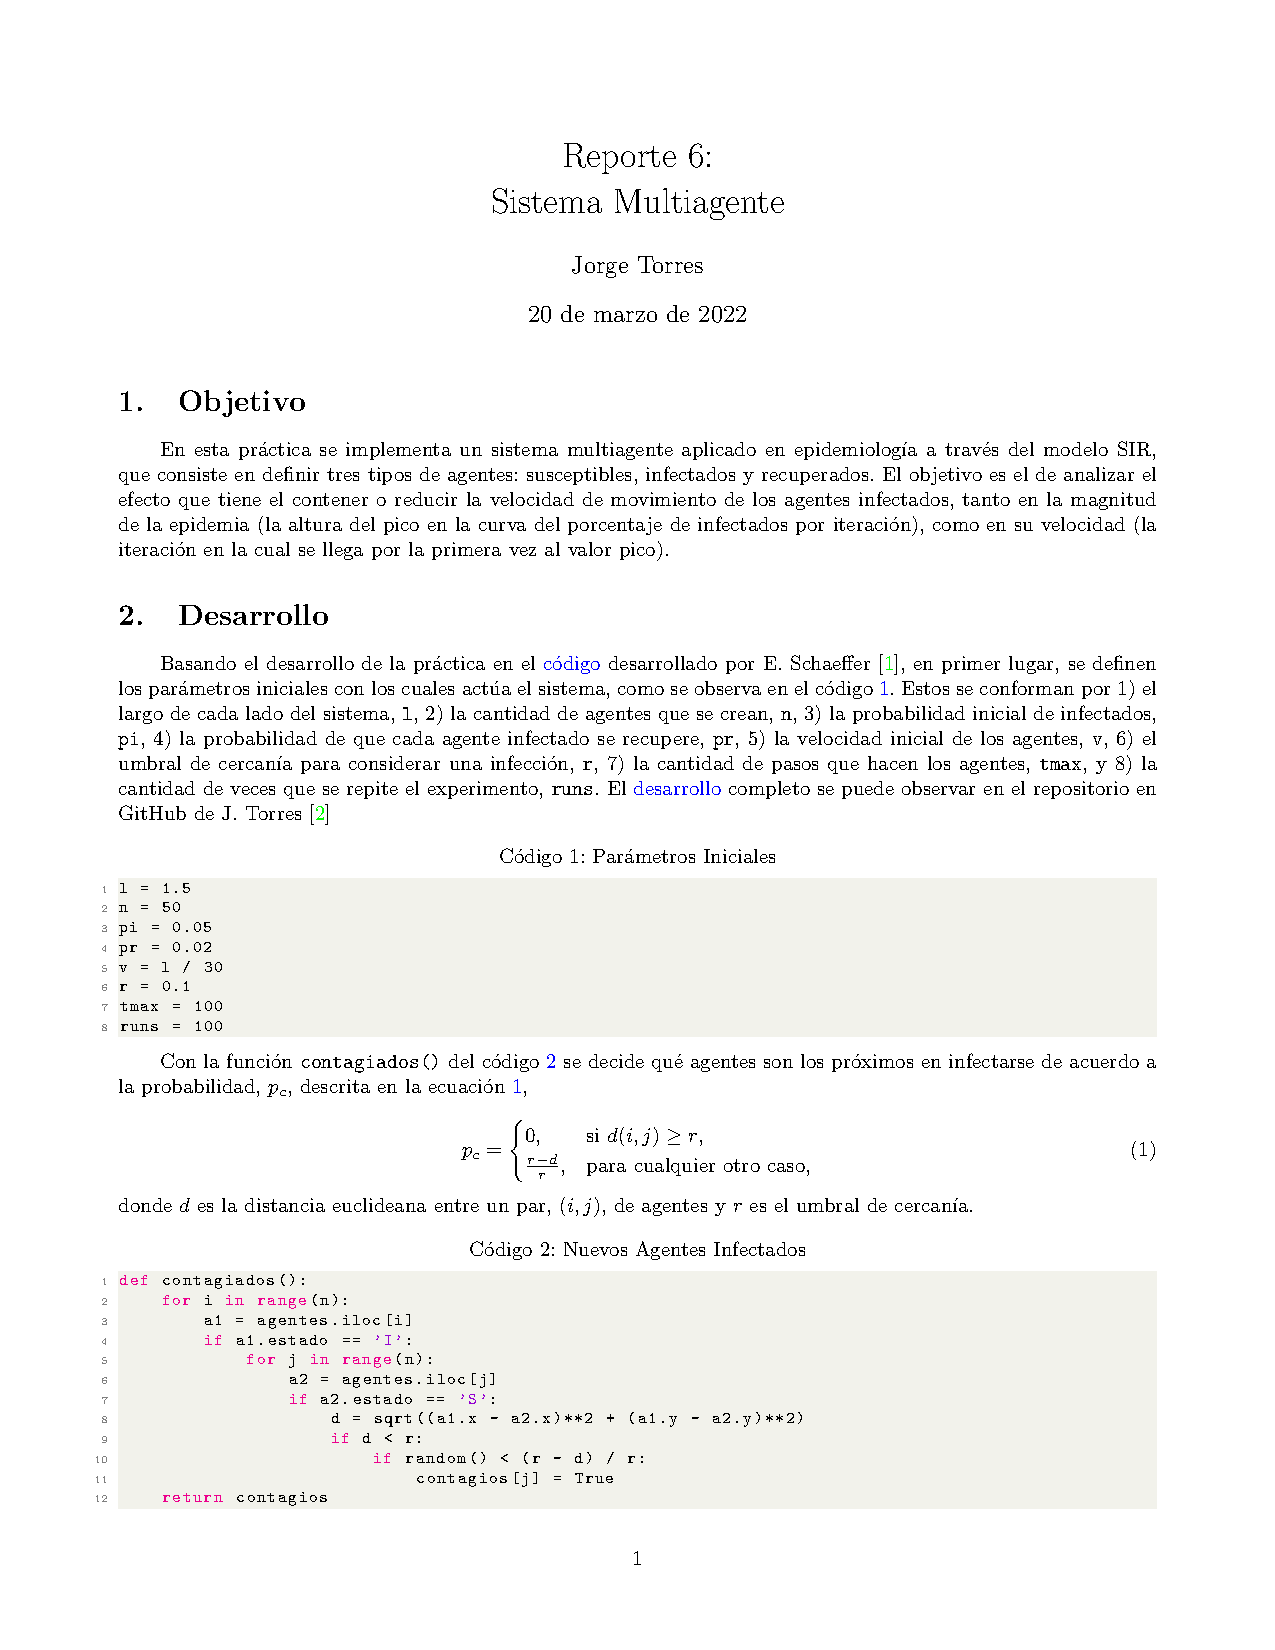
\includepdf[pages=-]{PDF_Tareas/Reporte_6.pdf}
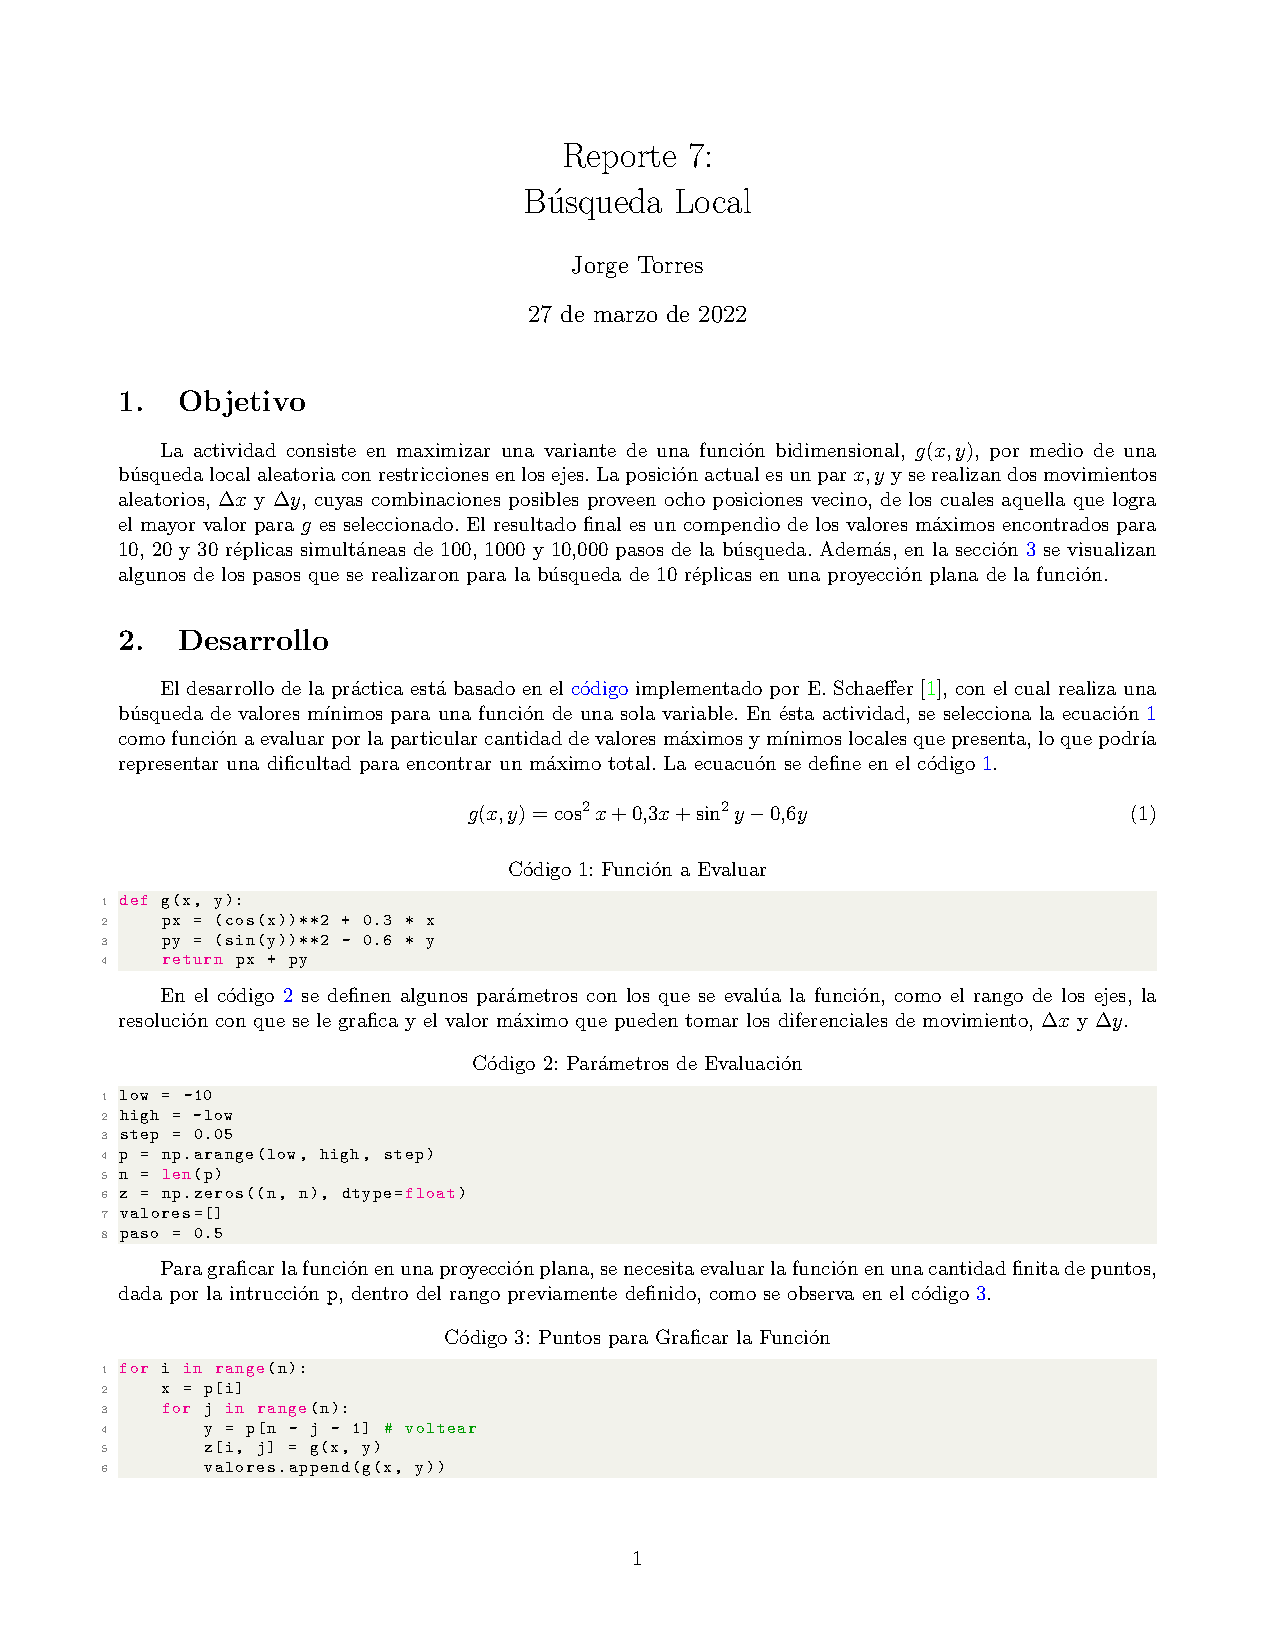
\includepdf[pages=-]{PDF_Tareas/Reporte_7.pdf}
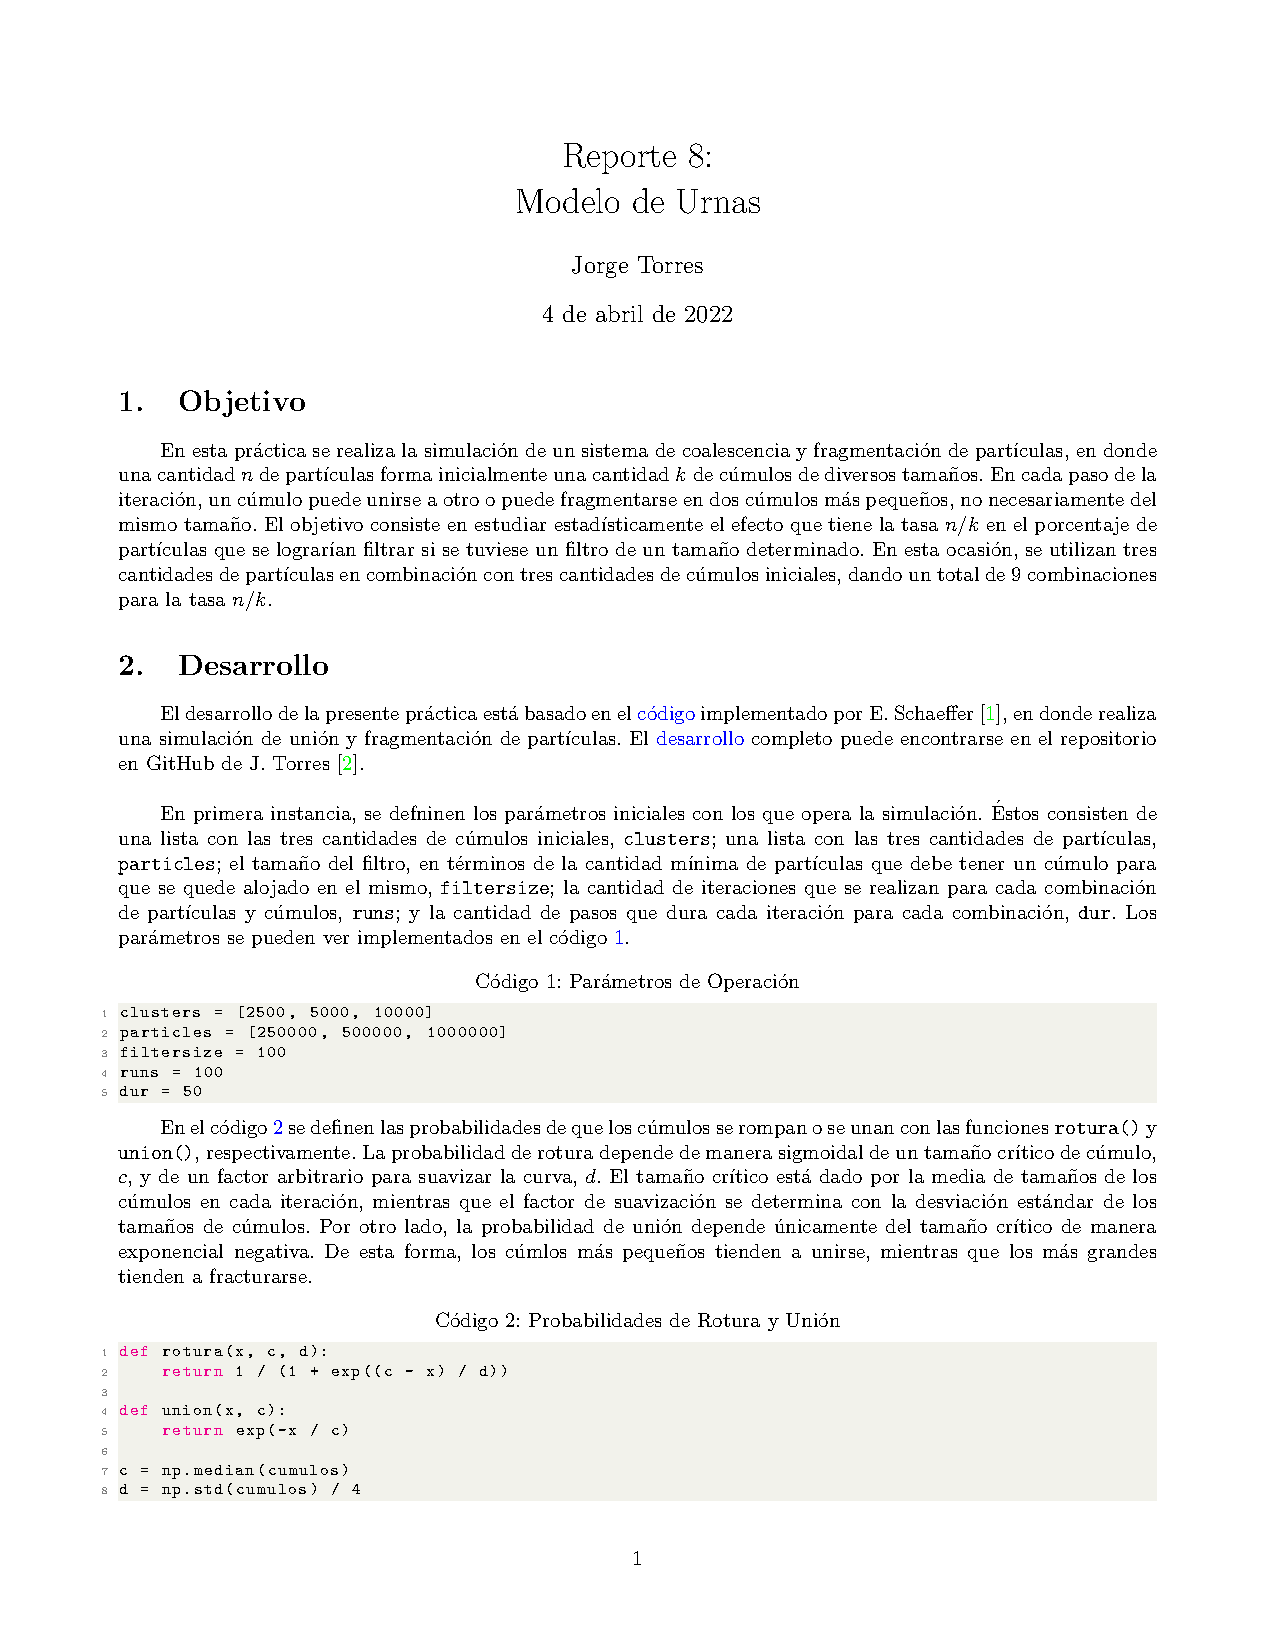
\includepdf[pages=-]{PDF_Tareas/Reporte_8.pdf}
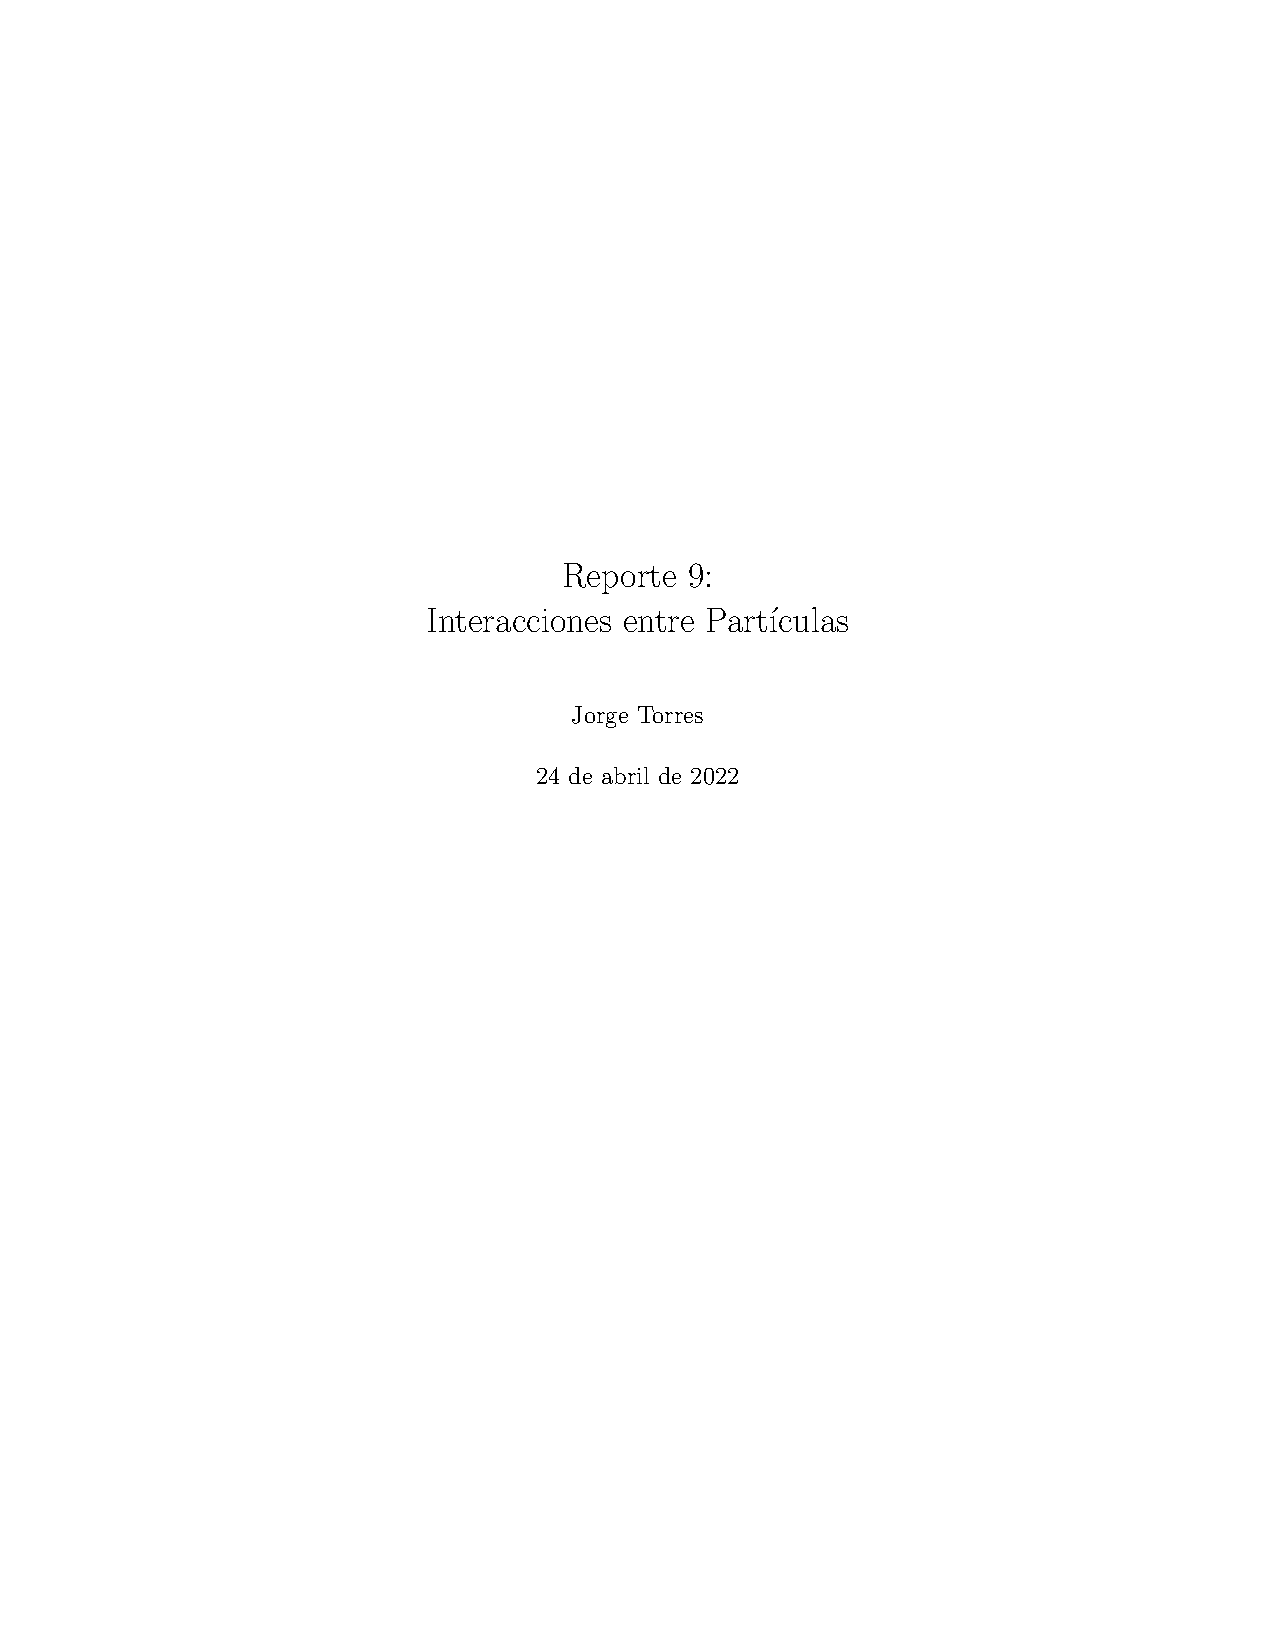
\includepdf[pages=-]{PDF_Tareas/Reporte_9.pdf}
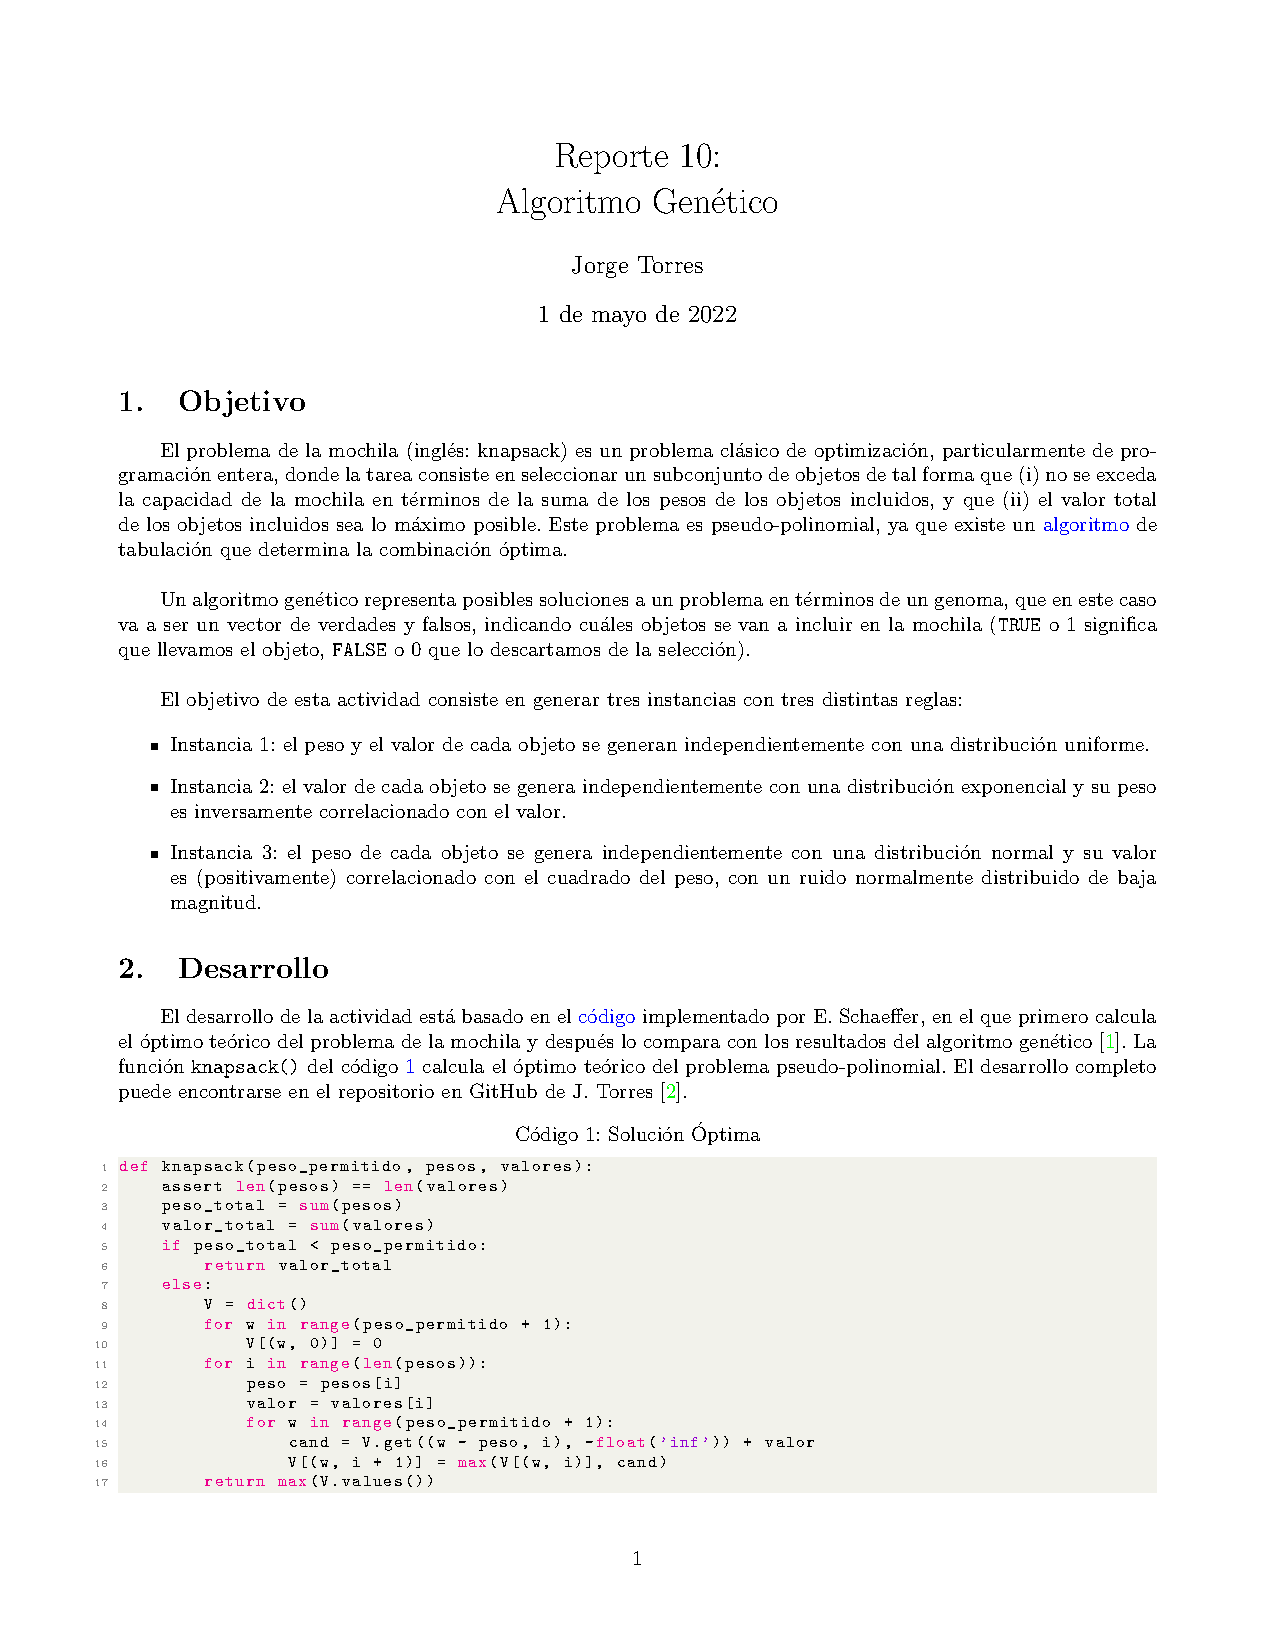
\includepdf[pages=-]{PDF_Tareas/Reporte_10.pdf}
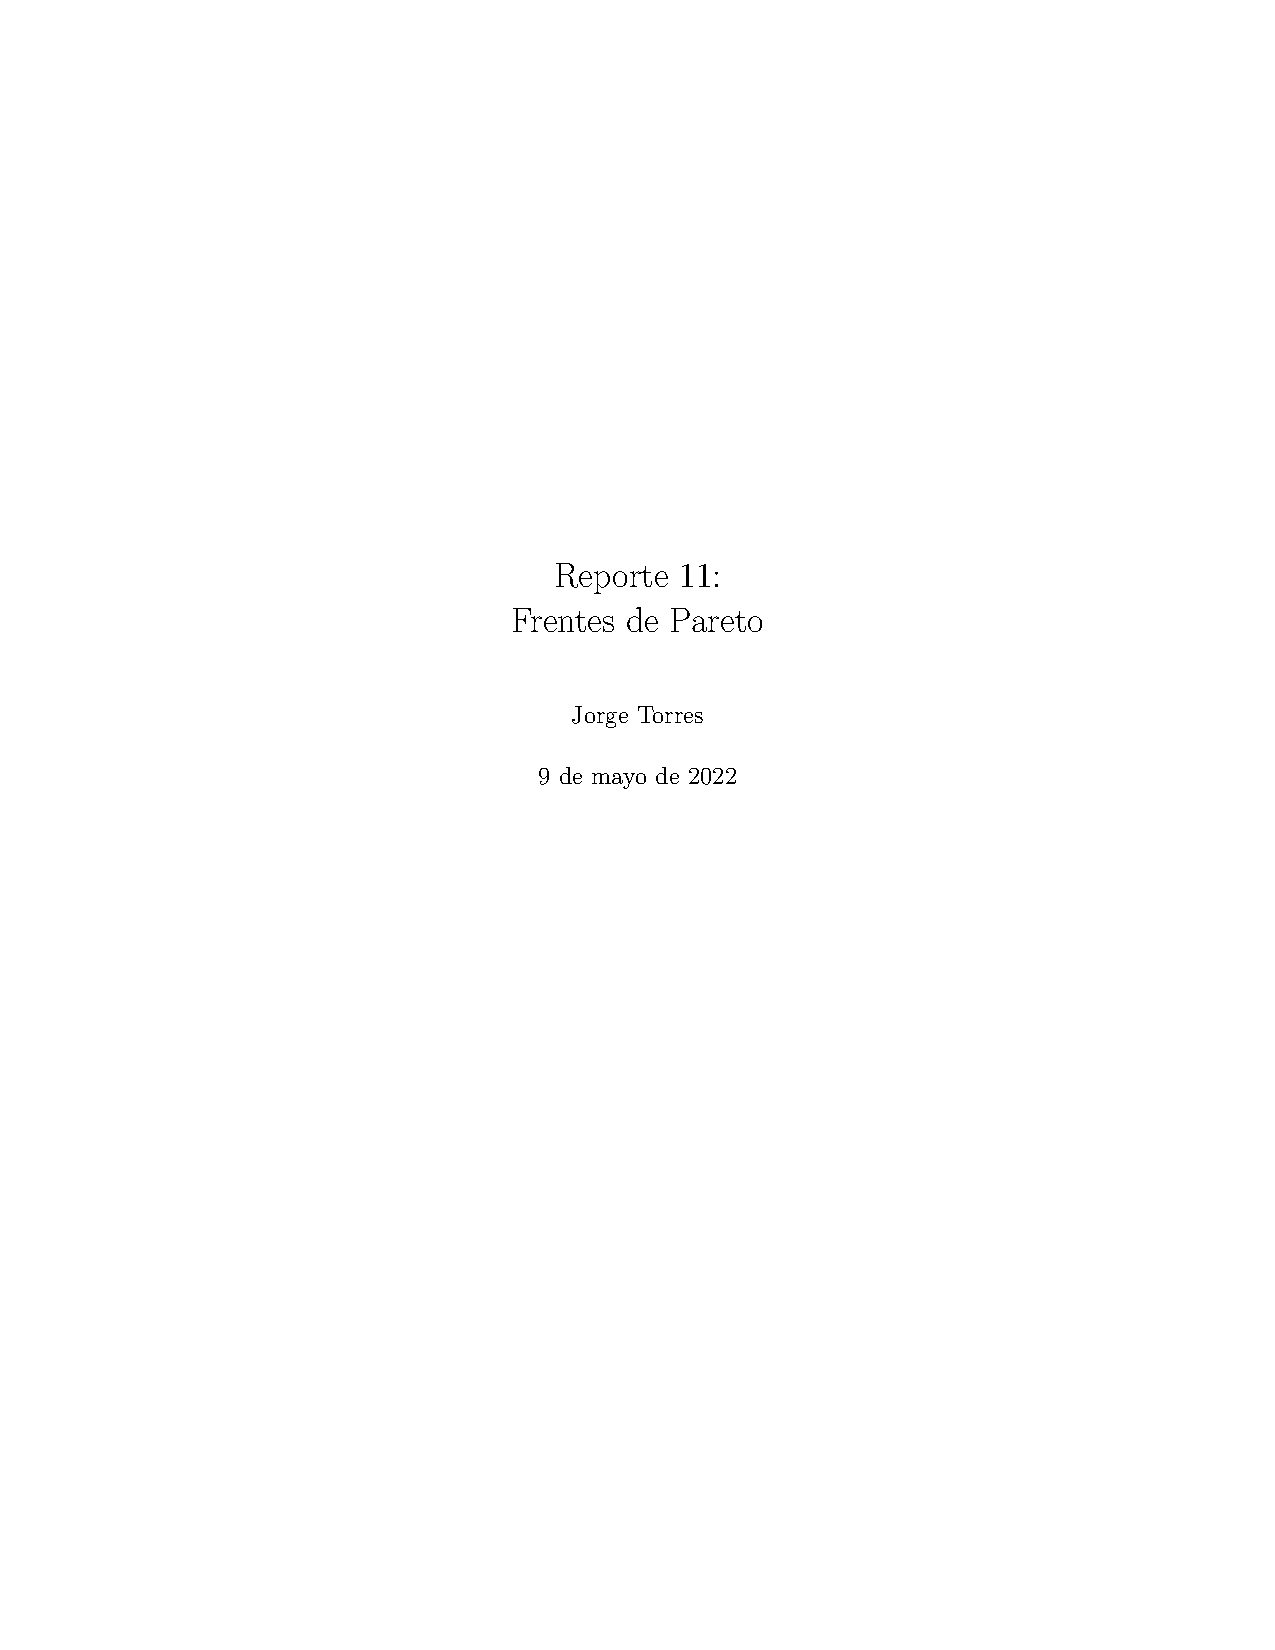
\includepdf[pages=-]{PDF_Tareas/Reporte_11.pdf}
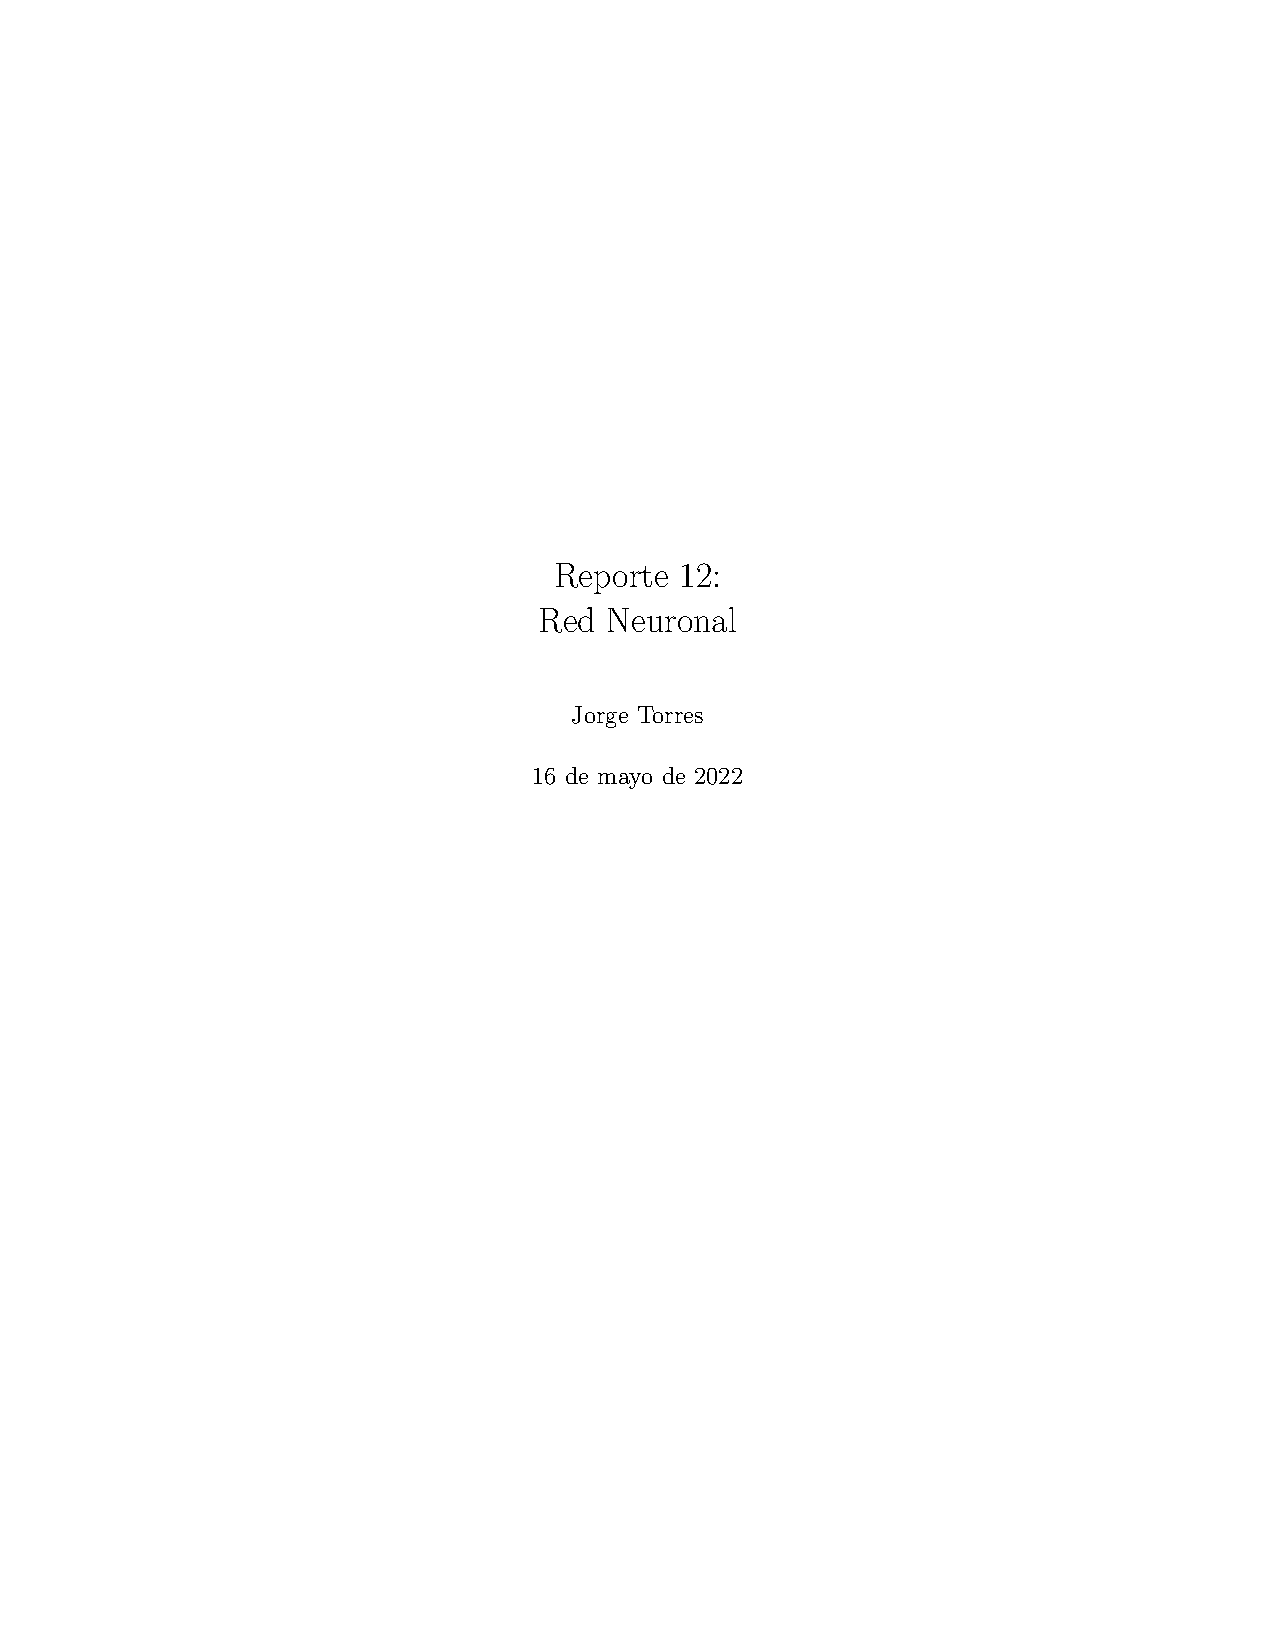
\includepdf[pages=-]{PDF_Tareas/Reporte_12.pdf}
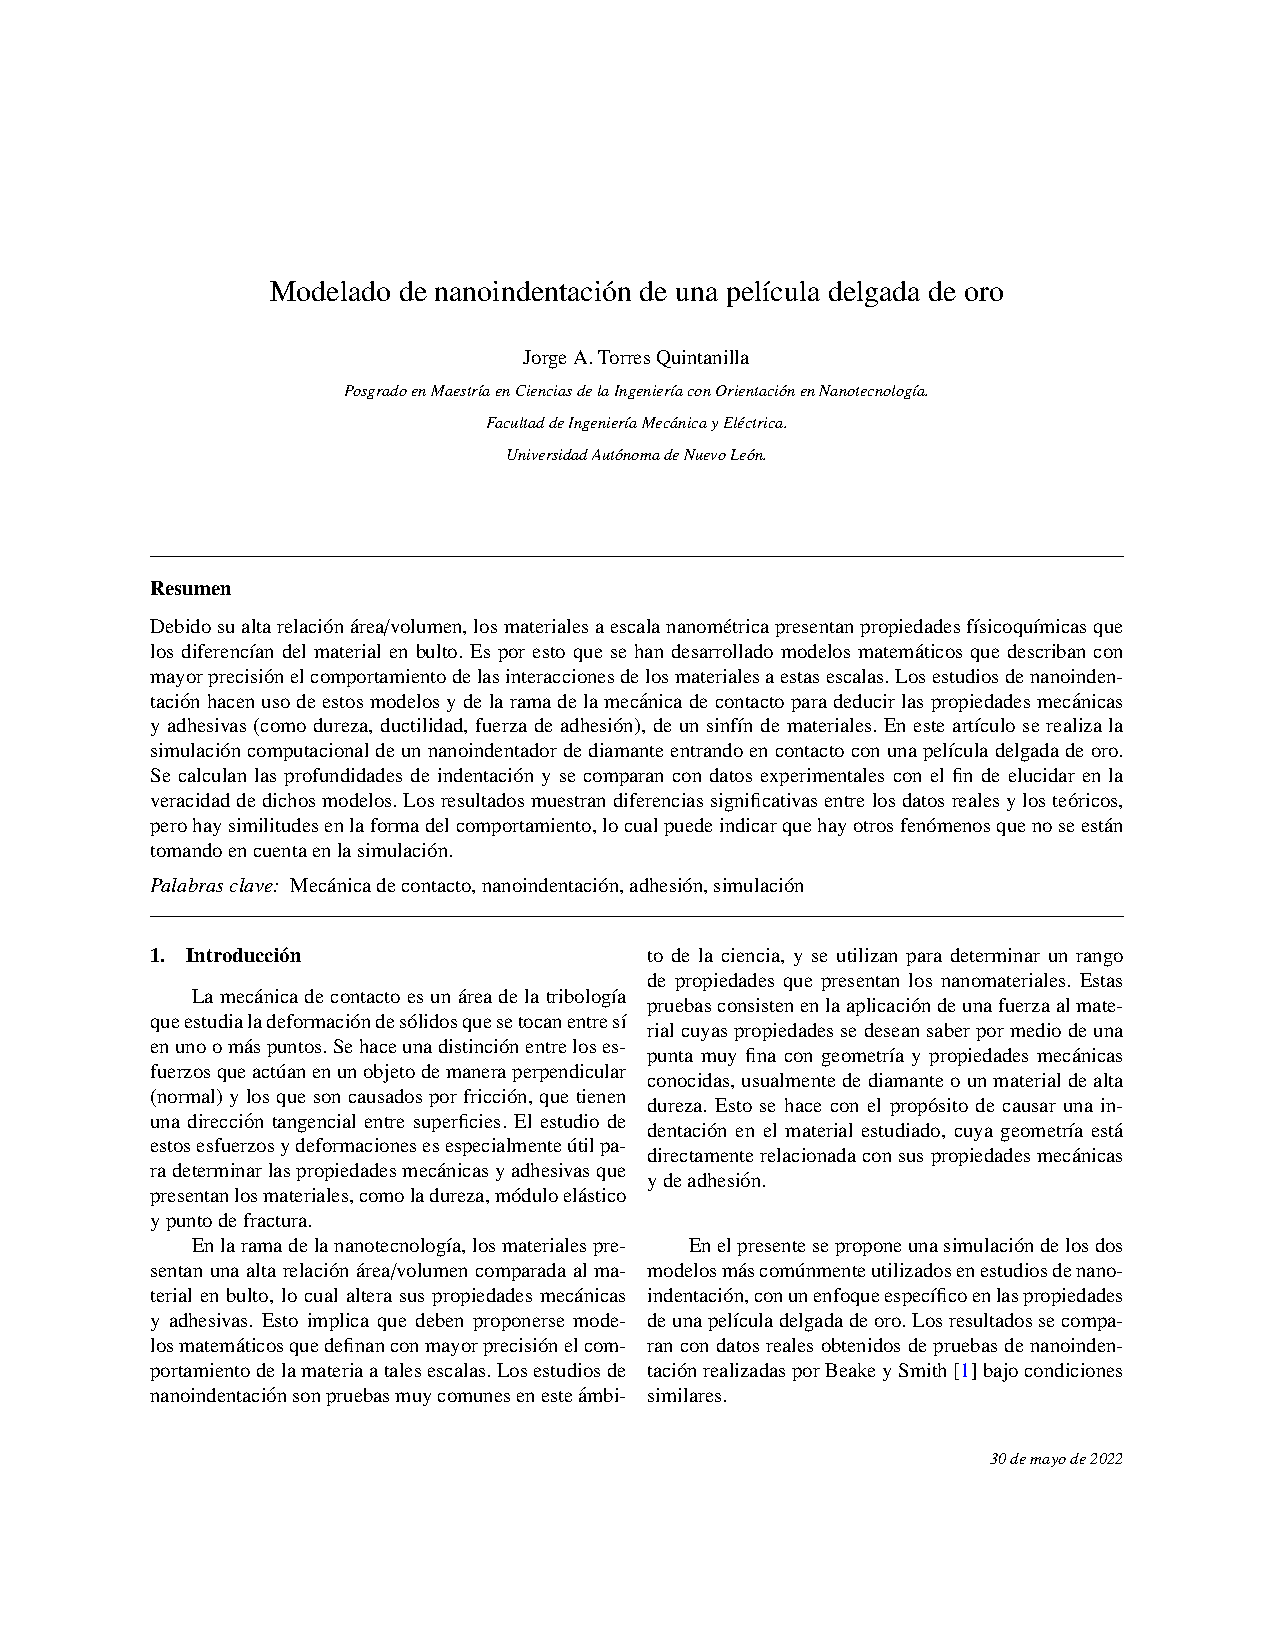
\includepdf[pages=-]{PDF_Tareas/Proyecto_Integrador.pdf}


\end{document}
